\begin{notation}[label={not:OpsFS}]{Notation for variables in the current section}
    In this section, we use the variable \( x \) to represent time and \( y \) to represent distance.
  \end{notation}

\subsection{Union, Intersection and Complement of Fuzzy Sets}
\signal{say why we assign those properties to the union and intersection to generalize the ones from classical sets}
\begin{definition}[Triangular Norm]
    A mapping $T:[0,1]\times [0,1] \longrightarrow [0,1]$ that satisfies:
    \begin{romanenum}
      \item \textbf{Symmetricity:} $T(x,y) = T(y,x) \quad \oldforall x,y \in [0,1]$
      \item \textbf{Associativity:} $T(x,T(y,z)) = T(T(x,y),z) \quad \oldforall x,y,z \in [0,1]$
      \item \textbf{Monotonicity:} $T(x,y) \leq T(x',y') \quad \textnormal{if }x\leq x' \textnormal{ and } y\leq y' \quad \oldforall x,y,x',y' \in [0,1]$
      \item \textbf{One Identity:} $T(x,1) = T(1,x) = x \quad \oldforall x \in [0,1]$
    \end{romanenum}
    is called a triangular norm or t-norm. Defines the \textbf{intersection} of two fuzzy sets $A$ and $B$ on $X$ by giving the membership function as $(A \cup B) (x) = T(A(x),B(x)) \forall x \in X$ 
\end{definition}

\begin{definition}[Triangular Conorm]
  A mapping $S:[0,1]\times [0,1] \longrightarrow [0,1]$ that satisfies:
  \begin{enumerate}[(i)]\setlength{\itemindent}{2em}
    \item \textbf{Symmetricity:} $S(x,y) = S(y,x) \quad \oldforall x,y \in [0,1]$
    \item \textbf{Associativity:} $S(x,T(y,z)) = S(S(x,y),z) \quad \oldforall x,y,z \in [0,1]$
    \item \textbf{Monotonicity:} $S(x,y) \leq S(x',y') \quad \textnormal{if }x\leq x' \textnormal{ and } y\leq y' \quad \oldforall x,y,x',y' \in [0,1]$
    \item \textbf{Zero Identity:} $S(x,0) = S(0,x) = x \quad \oldforall x \in [0,1]$
  \end{enumerate}
  is called a triangular conorm or t-conorm. Defines the \textbf{union} of two fuzzy sets $A$ and $B$ on $X$ by giving the membership function as $(A \cap  B) (x) = S(A(x),B(x)) \forall x \in X$ 
    
\end{definition}

\begin{definition}[Complement]
    The complement of a fuzzy set $A\in \fuzzy{X}$ is another fuzzy set with membership function given by $^\lnot A(x) \coleq 1 - A(x) \forall x\in X$
\end{definition}

Notice that this definition of complement is consistent with the classical definition of complement but implies that an element might have \textbf{non-zero partial membership} to both a fuzzy set and its complement: Let $A$ be a fuzzy set on $X$ and $x \in X / A(x)\notin \{0,1\}$ then $\lnot A(x)= 1 - A(x) \notin \{0,1\}$.\\

This implies as well that the union of a fuzzy set and its complement is not the total set in general. Analogously, the intersection will not the empty set in general. Those two properties that hold in classical sets, are often called the \textbf{laws of excluded middle and of non-contradiction}, respectively.\\

However, there is a particular t-norm and t-conorm (named after Lukasiewicz) that does satisfy both laws. This will have implications for the derived logic that will be explained in section \ref{sec:fuzzy_logic}. \signal{is it the only one?}

\hspace{10em}$T_L(x,y)=\max\{x+y-1,0\},\, S_L(x,y)=\min\{1,x+y\}$\\

Another important property that classical union and intersection satisfy is De Morgan's Laws. For an arbitrary pair of t-norm and t-conorm they are not satisfied but by imposing it, we get that the t-norm induces a t-conorm and viceversa.

\begin{proposition}[Relationship between t-norm and t-conorm]
  Given a t-norm $T$, the t-conorm $S(a,b)\coleq 1 - T(1-a, 1-b)$, then the union and intersection defined by that pair satisfy the De Morgan's Laws.
\end{proposition}
\begin{remark}
  It is easy to see that the previous relation is equivalent to $T(a,b) = 1-S(1-a, 1-b)$ which can be obtained simply by substituting $a'=1-a$ and $b'=1-b$, i.e., working with the complementary fuzzy sets.
\end{remark}

\begin{proof}
  Let $x\in X$, $A$, $B$ be fuzzy sets over $X$ with $a \coleq A(x)$ and $b \coleq B(x)$\\

  $\quad \boxed{\text{not}(A \text{ or } B) = (\text{not } A) \text{ and } (\text{not } B)}$\\[0.5em]
  $\lnot S(a,b) = T(\lnot a, \lnot b) \implies 1 - S(a,b) = T(1-a, 1-b) \implies S(a,b) = 1 - T(1-a, 1-b)$\\

  $\quad \boxed{\text{not}(A \text{ and } B) = (\text{not } A) \text{ or } (\text{not } B)}$\\[0.5em]
  $\lnot T(a,b) = S(\lnot a, \lnot b) \implies 1 - T(a,b) = S(1-a, 1-b) \implies T(a,b) = 1 - S(1-a, 1-b)$

\end{proof}

\signal{
  Lo de archimedean tiene el teorema 1.8.1 de Fuller 2. Y tb con la law of large numbers con LR-fuzzy numbers.
\begin{definition}[Archimedean t-norm]
  A continuous t-norm that satisfies $T(x,x)<x \forall x\in ]0,1[$ is called an archimedean t-norm.
\end{definition}

\begin{proposition}[Characterization of archimedean t-norms]
  For all archimedean t-norms there exists a continuous decreasing function $f:[0,1] \longrightarrow [0,\infty[$ with $f(1)=0$ such that: 
  \[ 
  T(x,y)= f^{-1}(\min\{f(x)+f(y), f(0)\}) \text{ where } f^{-1} =
  \begin{cases}
    f^{-1}(y) & \text{if } y\in [0,f(0) ]\\
    0 & \text{otherwise}
  \end{cases}
  \text{ is a pseudo-inverse}.
  \]
\end{proposition}
}

\signal{
\begin{definition}[Nilpotent t-norm]
  
\end{definition}}

\begin{definition}[Weaker t-norm]
  Given $T_1, T_2$ t-norms, then $T_1$ is weaker than $T_2$ $(T_1 \leq T_2)$ if $T_1(x,y)\leq T_2(x,y)\forall x,y\in [0,1]$.\\
  In that case, it is equivalent to say $T_2$ is stronger than $T_1$ $(T_2 \geq T_1)$

\end{definition}
\begin{remark}
  This defines a partial order relation in the set of t-norms.
\end{remark}
\signal{The weaker the t-norm, the stronger the associated s-norm? (not proved in Fuller)}

\signal{
There are many results like all t-norms are between the weak and the min, all t-conorms are between max and strong, or that min is the only t-norm that satisfies $T(a,a)=a$ (igual es por esto ultimo q se usa tanto. Qué implicaciones tiene que lukasiewicz no cumpla eso?)}

\signal{Tambien lo de que la T-norm e dsitributiva con max/sup sirve para justificar la definicion del producto cartesiano.}

\begin{example}
  \signal{Some examples of t-norms and t-conorms.}
\end{example}



\subsection{Fuzzy Relations}
\signal{Igual esto motivar la definición de relación con un ejemplo a estas alturas es pasarse?}

In the previous sections we have been working with a single domain denoted by $X$. Intuitively, it might be useful to think about the domain as the possible values of a property independently of the object that has that property. For example, we could say that for the property \textit{lenght} the domain is $\R^+\coleq
\{x\in\R \min x \geq 0\}$ and a person might have a \textit{height} defined in that domain (modeled as a fuzzy subset), although not all possible lengths values will be part of the support of a person's height since it is save to assume impossible to be 10 meters tall. If we were to look at the arm length, then we would have another subset of the lenghts. Treating each subset independently, doesn't allow to distinguish between the people of the same height with different arm lenght or viceversa. Therefore it is needed to a way to differentiate each unique combination of attributes. Notice that in this example, height and arm length have the same domain but for example hair color would have a different domain.\\

Mathematically, this is done with \textbf{relations} which are subsets of the cartesian product of the domains, so that each element is a unique possible combination of attributes, an ordered n-tuple. For simplicity, let us consider just the cartesian product of 2 sets since the general case can be obtained inductively. Again, the "fuzzy" part will be referred to how we generalize the membership values to the continuum.\\


\begin{definition}[Fuzzy Relation]
  Let $X\neq \emptyset \neq Y$ be classical sets. Then a fuzzy relation $R$ is a fuzzy set on $X\times Y$, i.e., $R\in \fuzzy{X\times Y}$. $R(x,y)$ will denote the degree of membership of $(x,y) \in R$
\end{definition}

\begin{notation}[label={not:compositionFS}]{Notation}
  Although Fuzzy Relations are Fuzzy Sets as well, we will often use the name distinction to denote whether the domain is a cartesian product or not.
\end{notation}

\begin{remark}
  To formally extend the Cartesian product from two sets to \( n \) sets using induction, it is important to observe that it satisfies associativity up to a natural isomorphism, i.e., 
  \[
  (A\times B)\times C \cong A\times (B\times C).
  \]
\end{remark}

Before giving the definition of the fuzzy cartesian product, we need to first understand what the classical cartesian product is in terms of the membership function. When we define a cartesian product $A\times B$ as "\textit{all unique ordered pairs of elements from $A$ \textbf{and} $B$}", in terms of membership functions we are taking the intersection of membership to $A$ and membership to $B$. Therefore, generalizing that notion with a t-norm we get the following definition.

\begin{definition}[Fuzzy Cartesian Product]
  It is a fuzzy relation $A\times B \in \fuzzy{X\times Y}$ such that the membership function is given by:
  \[ 
  (A\times B)(x,y) = T(A(x), B(y)), \quad \forall (x,y) \in X\times Y
  \]
  where $T$ is a t-norm.
\end{definition}

To justify the definition of the membership function of a cartesian product of two fuzzy sets, let us first recall that in classical sets, we can retrieve the orginal subsets individually by taking the projection of the cartesian product. Given $R$ a relation on $X\times Y$ the projections are:

\[\Pi_X(R)=\{x \in X \mid \exists y \in Y \textnormal{ such that } (x,y) \in R\}\]
\[\Pi_Y(R)=\{y \in Y \mid \exists x \in X \textnormal{ such that } (x,y) \in R\}\]

Then, with the boolean membership, it can be expressed as well as:

\[\Pi_X(R)(x)=\sup\{R(x,y) \mid y\in Y\}=
\begin{cases}
  1 & \textnormal{if } \exists y \in Y \textnormal{ such that } (x,y) \in R \\
  0 & \textnormal{otherwise}
\end{cases}
\]
\[
  \Pi_Y(R)(y)=\sup\{R(x,y) \mid x\in X\}=
  \begin{cases}
    1 & \textnormal{if } \exists x \in X \textnormal{ such that } (x,y) \in R \\
    0 & \textnormal{otherwise}
  \end{cases}
\]

It is clear that in the case of having 2 possible values for the membership function, the above expresions are identical. The use of $\sup$ in the definition of the projection can be intuitively interpreted as the \textit{shadow} of the membership function of the cartesian product, as figure \ref{fig:class_cart_prod} illustrates. It is also desirable because then the following property holds for any classical \signal{(and fuzzy?)} cartesian product:\\
$$ 
\Pi_X(A\times B)=A \quad \textnormal{ and } \quad \Pi_Y(A\times B)=B \forall A\in X, \forall B \in Y
$$

\begin{figure}[ht]
  \centering
  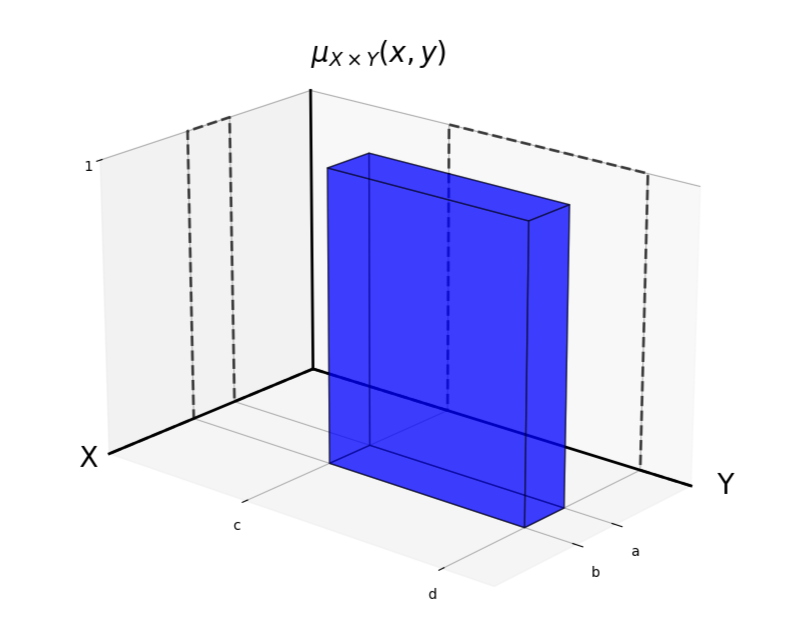
\includegraphics[width=0.65\textwidth]{ch1/figures/class_cart_prod.png}
  \caption{The blue volume represents the membership function of the cartesian product of two classical sets $X=[a,b]$ and $Y=[c,d]$ in $\R$. In the plane $y=0$ we have the projection that corresponds to the membership function of $X$ and analogously, the projection of $Y$ in the plane $x=0$.}
  \label{fig:class_cart_prod}
\end{figure}

Therefore, we define:

\begin{definition}[Projection of a fuzzy relation]
  The projection from fuzzy relations on $X\times Y$ onto the fuzzy sets on $X$ is the function:
  \[
    \begin{aligned}
      \Pi_X: \fuzzy{X\times Y} &\longrightarrow \fuzzy{X} \\
      R &\longmapsto \Pi_X(R)
    \end{aligned}
  \]
  where $\Pi_X(R)(x) = \sup_{y\in Y}\{R(x,y)\}\forall x \in X$
\end{definition}

Applying the definition of projection with the supremum to fuzzy sets, we have a way to retrieve the membership function of each fuzzy set given the membership function of a fuzzy cartesian product (figure \ref{fig:fuzzy_cart_prod}). \\






\begin{figure}[ht]
    \centering
    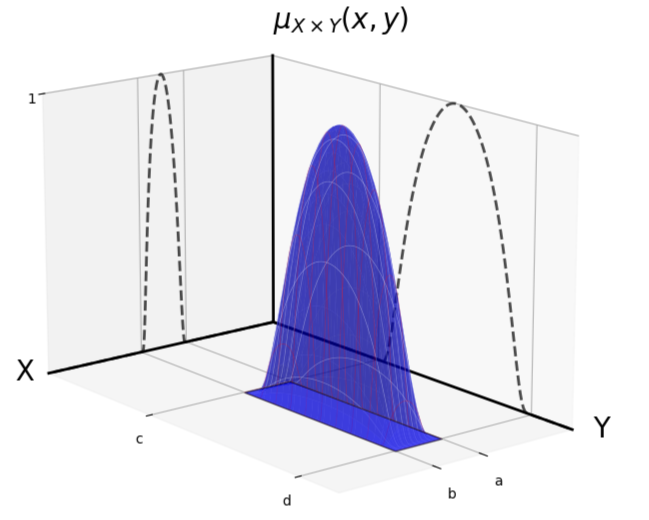
\includegraphics[width=0.65\textwidth]{ch1/figures/fuzzy_cart_prod.png}
    \caption{The blue volume represents the membership function of the cartesian product of two fuzzy sets $X$ and $Y$. In the plane $y=0$, we have the projection that corresponds to the membership function of $X$, and analogously, the projection of $Y$ in the plane $x=0$. The partial memberships illustrate how the fuzzy relations can vary across the domains.}
    \label{fig:fuzzy_cart_prod}
\end{figure}

\signal{Falta ver que que la proyección nos devuelve el fuzzy set original en los fuzzy cart prod.}

\subsubsection*{Composition of Fuzzy Sets}

% The definition of projection allows us to define a composition of fuzzy relations with a common domain. Intuitively, a composition is the projection into the uncommon domain of the intersection of each fuzzy relation.

% \begin{definition}[Composition of 2 Fuzzy Relations]
%     Let $R\in \fuzzy{X\times Y}$, $G \in \fuzzy{X\times Y}$ be 2 fuzzy relations with one of the sets of the domain in common. Then the composition is another fuzzy relation $R\circ G\in \fuzzy{X\times Z}$ (the non common sets of the domain) and the membership function is given by the projection of the cartesian product:
%     \[
%     (R \circ G) (x,z) = \Pi_{X\times Z}[T(R(x,y), G(y,z))] = \sup_{y\in Y}\{T(R(x,y), G(y,z))\}
%     \]
% \end{definition}

The concept of projection allows us to combine fuzzy relations sharing a common domain. Intuitively, composing two fuzzy relations involves intersecting their membership values (using a t-norm) and then projecting the result onto the domain where the relations do not overlap.

\begin{definition}[Composition of Two Fuzzy Relations]
    Let \( R \in \fuzzy{X \times Y} \) and \( G \in \fuzzy{Y \times Z} \) be fuzzy relations sharing the set \(Y\). Their composition \( R \circ G \) is the fuzzy relation in \(\fuzzy{X \times Z}\) defined by
    \[
    (R \circ G)(x,z) = \Pi_{X\times Z}\Bigl[\, T\bigl(R(x,y), G(y,z)\bigr) \Bigr] = \sup_{y\in Y}\, T\bigl(R(x,y), G(y,z)\bigr),
    \]
    where \(T\) is a t-norm acting as the fuzzy intersection.
\end{definition}

% This means that given three properties $X$, $Y$ and $Z$ and two fuzzy relation R from X to Y and another fuzzy relation from Y to Z, we have a way to induce a relation $R\circ G$ between X and Z.

% (add a diagram here)

Given three sets \(X\), \(Y\), and \(Z\), suppose we have a fuzzy relation \(R\) from \(X\) to \(Y\) and another fuzzy relation \(G\) from \(Y\) to \(Z\). Using the composition operation, we can derive a new fuzzy relation \(R \circ G\) that directly connects \(X\) to \(Z\).

\noindent
\begin{minipage}{0.7\textwidth}
In this diagram, the arrows represent fuzzy relations, with \(R\) mapping elements from \(X\) to \(Y\), \(G\) mapping from \(Y\) to \(Z\), and \(R \circ G\) representing the induced fuzzy relation between \(X\) and \(Z\) through composition.\\
\end{minipage}%
\begin{minipage}{0.3\textwidth}
  \begin{center}
    \begin{tikzcd}
      X \arrow[r, "R", leftrightarrow] & Y \arrow[r, "G", leftrightarrow] & Z \arrow[bend right=30, from=1-1, "R \circ G"', leftrightarrow]
      \end{tikzcd}
  \end{center}

\end{minipage}


We can define a the composition of a fuzzy set with a fuzzy relation in a completely analogous way. 

\begin{definition}[Composition of a Fuzzy Set and a Fuzzy Relation]
    Let \( A \in \fuzzy{X} \) be a fuzzy set on \(X\) and \( R \in \fuzzy{X \times Y} \) be a fuzzy relation between \(X\) and \(Y\). The composition \( A \circ R \in \fuzzy{Y} \) is defined by
    \[
    (A \circ R)(y) = \Pi_{Y}\Bigl[\, T\bigl( A(x), R(x,y) \bigr) \Bigr] = \sup_{x \in X}\, T\bigl( A(x), R(x,y) \bigr),
    \]
    where \(T\) is a t-norm.
\end{definition}



\subsection{Extension Principle}

Following a similar idea as in the definition of the composition of fuzzy sets, we can derive a way to generalize crisp functions \signal{(Hasta ahora lo he llamado classical en vez de crisp, tengo que explicarlo y elegir una notación uniforme)} to fuzzy sets.\\

Let's consider the crisp function $f:\,X \longrightarrow Y$ where $X$ and $Y$ are classical sets. And consider as well the fuzzy sets $A \in \fuzzy{X}$. Then $f$ induces the classical relation $R=\{(x,y)\in X\times Y \mid f(x)=y\}$. And we can also make this relation fuzzy by copying the membership function of $A$:
$$ \mu_R (x,y) = \mu_A (x) \forall (x,y)\in R$$
Now we can define $B\in\fuzzy{Y}$, the fuzzy image of $A$ under $f$, as the projection of this fuzzy relation:
$$\mu_B (y) = \Pi_Y (R) = \sup\{R(x,y)\mid x\in X\} = \sup\{\mu_A (x)\mid x\in X, \, f(x)= y\} = \sup_{x\in f^{-1}(y)}\{\mu_A(x)\}$$

This is called the (Zadeh's) extension principle and is the basis for building arithmetic for fuzzy numbers (see section \ref{sec:fuzzy_numbers}) and generalizing any crisp function to fuzzy sets: 

\begin{definition}[Zadeh's extension principle]
  Let $f: X \longrightarrow Y$ be a crisp function and $A\in \fuzzy{X}$ a fuzzy set on $X$. Then we can define $f(A)\in \fuzzy{Y}$ as:
  \[
  \mu_{f(A)}(y)\equiv f(A)(y) = 
  \begin{cases}
    \sup_{x\in f^{-1}(y)}A(x) & \textnormal{if } f^{-1}(y)\neq \emptyset\\
    0 & \textnormal{otherwise}
  \end{cases}
  \quad\quad\quad \textnormal{where } f^{-1}(y)=\{x\in X \mid f(x)=y\}
  \]
\end{definition}


\begin{remark}
  If $f$ is \textbf{injective} then for any $y \in \textnormal{Im}(f)$ there exists a unique $x \in X$ such that $f(x)=y$, and therefore $f^{-1}(y)=\{x\}$. Then the first case can be rewritten as, $f(A)(y) = A(f^{-1}(y))$ if $y \in \textnormal{Im}(f)$.
\end{remark}

It is important to highlight as well that this definition is straight forward generalization of set-valued functions where $f(A)= \{f(x)\mid x\in A\}$. In terms of boolean membership function:
$$\chi _{f(A)}(y)=\sup_{x\in f^{-1}(y)}\chi_A(x)$$

The definition above can be generalized to vector functions using the definition of fuzzy cartesian product, which requires us to take the intersection:

\begin{definition}[Sup-T extension principle]
  Let $f: X_1 \times \cdots \times X_n \longrightarrow Y$ be a crisp function and $A_1 \in \fuzzy{X_1}, \ldots, A_n \in \fuzzy{X_n}$ be fuzzy sets. Then we can define $f(A_1,\ldots,A_n)\in \fuzzy{Y}$ as:
  \[
  \mu_{f(A_1,\ldots,A_n)}(y)\equiv f(A_1,\ldots,A_n)(y) = 
  \begin{cases}
    \sup_{(x_1,\ldots,x_n)\in f^{-1}(y)} T(A_1(x_1),\ldots,A_n(x_n)) & \textnormal{if } f^{-1}(y)\neq \emptyset\\
    0 & \textnormal{otherwise}
  \end{cases}
  \]
  where $f^{-1}(y)=\{(x_1,\ldots,x_n)\in X_1\times\cdots\times X_n \mid f(x_1,\ldots,x_n)=y\}$ and $T$ is a t-norm.
\end{definition}

Which is again a generalization of vector set-valued functions where: $$f(A_1,\ldots,A_n)= \{f(x_1,\ldots,x_n)\mid x_i\in A_i\}$$
In terms of boolean membership function:
$$\chi _{f(A_1,\ldots,A_n)}(y)=\sup_{(x_1,\ldots,x_n)\in f^{-1}(y)}T(\chi_{A_1}(x_1),\ldots,\chi_{A_n}(x_n)) = \sup_{(x_1,\ldots,x_n)\in f^{-1}(y)}min\{\chi_{A_1}(x_1),\ldots,\chi_{A_n}(x_n)\}$$

Where we have used that every t-norm operates the same on boolean memberships. \signal{Debería haber puesto esto como un remark cuando presento la intersección y la unión.}\\

\signal{Hay otros principios de extensión como el de Ramik con extensiones canónicas y order preserving operators, etc. No sé hasta qué punto eso podrá serme útil.}